\chapter{Metode Penelitian}

\section{Alat dan Bahan Tugas akhir}

\subsection{Alat Tugas akhir}

Alat-alat yang digunakan dalam tugas akhir ini terdiri atas perangkat keras dan perangkat lunak sebagai berikut:

\begin{enumerate}
	\item Laptop Lenovo IdeaPad Slim 3 (Model 82K2) dengan sistem operasi Windows 11 Home Single Language 64-bit. Laptop ini dilengkapi prosesor AMD Ryzen 5 5600H with Radeon Graphics berarsitektur 64-bit dengan 6 core dan 12 thread, memori utama sebesar 8 GB RAM, serta grafis terintegrasi AMD Radeon Graphics.
	Laptop ini digunakan untuk pengolahan data, pemrograman, dan pengembangan web.
	\item Visual Studio Code versi 1.125.1 digunakan sebagai IDE untuk menulis, menjalankan, dan mengelola kode Python berbasis \textit{Jupyter Notebook (.ipynb)}, mencakup pra-pemrosesan data, pembangunan graf jaringan sanad, perhitungan sentralitas perawi, dan pengembangan \textit{front-end}.
	\item Python versi 3.13.13 digunakan sebagai bahasa pemrograman utama dalam pembersihan dan pengolahan data.
	\item Pustaka NetworkX versi 3.6.1 digunakan untuk membangun graf dan menghitung sentralitas jaringan perawi.
	\item JavaScript adalah bahasa pemrograman yang digunakan untuk membuat halaman web menjadi dinamis, interaktif, dan responsif.
	\item React versi 18.3.1 adalah \textit{library} JavaScript untuk membangun komponen UI yang dapat digunakan ulang (\textit{reusable}) dan efisien dalam merender ulang tampilan saat data berubah, cocok untuk \textit{dashboard} dengan data dinamis.
	\item Supabase digunakan sebagai backend dan database aplikasi, menyediakan penyimpanan data, autentikasi pengguna, dan API secara otomatis.
\end{enumerate}

\subsection{Bahan Tugas akhir}
Bahan yang digunakan adalah data hadis dari studi Mghari \textit{et al} \cite{MGHARI2022108540}, bersifat statis dalam format CSV (\textit{Comma-Separated Values}), terdiri atas:

\begin{itemize}
	\item \texttt{sanadset.csv} memuat lebih dari 650.986 rekaman hadis yang bersumber dari 926 kitab hadis Arab klasik, dengan masing-masing rekaman terdiri atas 6 variabel yang mencakup informasi kitab asal, nomor hadis, teks hadis, Matn, daftar perawi, dan jumlah perawi.

	\item \texttt{hadith\_samples.csv} berisi sepuluh contoh hadis dalam bahasa Arab untuk membantu pemahaman format dan struktur data sebelum pengolahan keseluruhan korpus.

	\item \texttt{translated\_samples.csv} memuat versi terjemahan bahasa Inggris dari sampel hadis yang tersedia. File ini memudahkan pemahaman isi hadis serta pembedaan komponen Sanad dan Matn, khususnya bagi peneliti yang tidak menggunakan bahasa Arab.

	\item \texttt{books.csv} mendokumentasikan daftar kitab klasik sumber data untuk menjaga ketertelusuran sehingga setiap hadis dapat dirujuk ke kitab asalnya.
\end{itemize}

Dari keempat file tersebut, \texttt{sanadset.csv} dipilih sebagai dataset utama karena memuat informasi perawi dan rantai sanad yang dibutuhkan untuk pembangunan graf jaringan sanad dan perhitungan sentralitas perawi.



\begin{figure}[H]
	\centering
	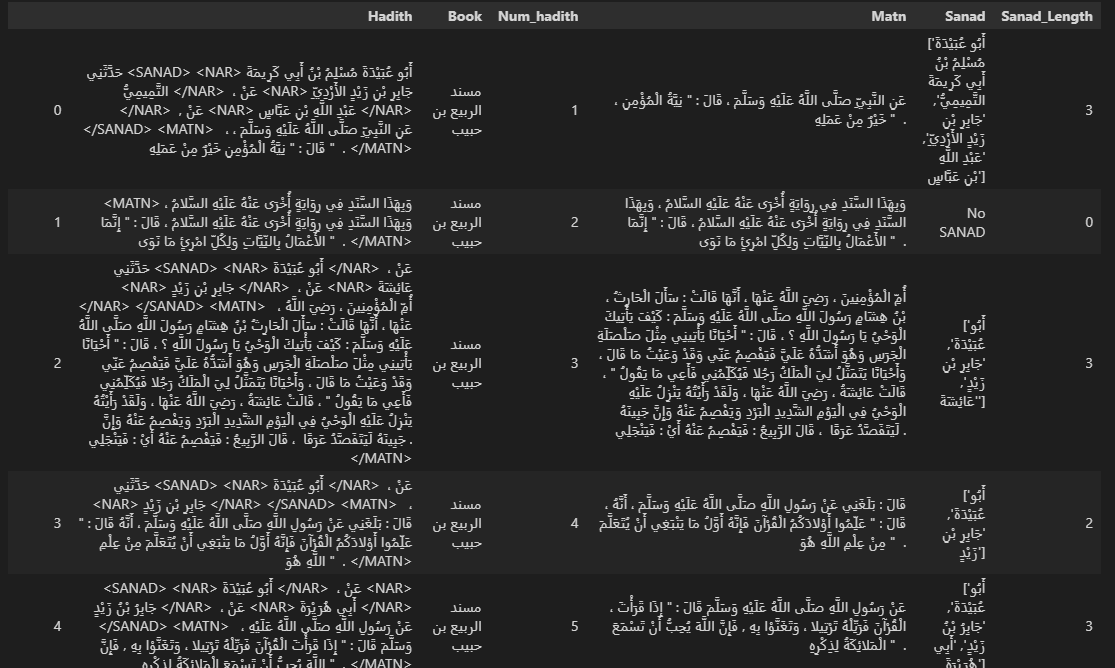
\includegraphics[width=\textwidth]{contents/chapter-3/data-sanadset.png}
	\caption{Contoh data pada \textit{sanadset.csv}}
	\label{fig:sanadset-preview}
\end{figure}

\section{Metode yang Digunakan}
\subsection{Pra Pemrosesan Data}
\subsubsection{Penghapusan baris tanpa sanad}
\begin{sloppypar}
Dataset mentah \texttt{sanadset.csv} yang digunakan dalam penelitian ini memuat 650.986 baris data hadis dari berbagai kitab hadis. Setiap baris merepresentasikan satu hadis dengan kolom-kolom: \texttt{Hadith}, \texttt{Book}, \texttt{Num\_hadith}, \texttt{Matn}, \texttt{Sanad}, dan \texttt{Sanad\_Length}.
Dalam proses pengumpulan data, tidak semua hadis dalam korpus memiliki rantai sanad yang teridentifikasi. Hadis-hadis tersebut ditandai dengan nilai \texttt{'No SANAD'} pada kolom \texttt{Sanad} dan nilai \texttt{0} pada kolom \texttt{Sanad\_Length}. Kondisi ini dapat disebabkan oleh beberapa hal, seperti hadis yang hanya memuat teks matn tanpa mencantumkan jalur periwayatan, atau hadis yang sanadnya tidak berhasil diekstraksi pada tahap anotasi dataset.
Hadis-hadis demikian tidak dapat dimodelkan sebagai relasi dalam graf jaringan sanad karena tidak memuat informasi perawi maupun hubungan antar-perawi. Oleh karena itu, seluruh baris dengan nilai \texttt{'No SANAD'} dihapus dari dataset menggunakan filter kondisional. Setelah proses ini, dataset yang tersisa berjumlah 491.428 baris, berkurang sebesar 159.558 baris atau sekitar 24,5\% dari total data awal. Seluruh data yang tersisa dipastikan memiliki rantai sanad yang dapat diproses pada tahap-tahap selanjutnya.
\end{sloppypar}

\subsubsection{Penghapusan Harakat (Tanda Baca Arab)}
\begin{sloppypar}
Tahap kedua adalah penghapusan harakat dari seluruh nama perawi dalam kolom \texttt{Sanad}. Teks Arab dalam dataset memuat harakat, yaitu tanda baca diakritik yang berfungsi sebagai penanda vokal dalam tulisan Arab, meliputi fathah, kasrah, dhammah, tanwin, sukun, dan tasydid. Dalam penulisan kitab hadis klasik, penggunaan harakat tidak seragam---nama perawi yang sama dapat muncul dengan harakat lengkap, sebagian, atau tanpa harakat sama sekali. Ketidakseragaman ini menyebabkan satu perawi yang sama diperlakukan sebagai entitas berbeda oleh sistem, sehingga memecah node yang seharusnya merepresentasikan satu perawi menjadi beberapa node terpisah dalam graf. Sebagai contoh, nama \textit{J\={a}bir ibn Zayd} yang ditulis dengan harakat lengkap dan tanpa harakat merujuk pada perawi yang sama, namun secara komputasional dianggap sebagai dua string berbeda apabila tidak dinormalisasi terlebih dahulu. Kondisi ini akan menghasilkan perhitungan sentralitas yang tidak akurat apabila dibiarkan.

Penghapusan harakat dilakukan dengan mengidentifikasi dan menghapus seluruh karakter diakritik Arab (harakat) tersebut menggunakan ekspresi reguler (\textit{regex}). Fungsi yang diimplementasikan mampu menangani input berupa string maupun \textit{list of string}, mengingat kolom \texttt{Sanad} menyimpan data dalam format daftar nama perawi. Hasil pembersihan disimpan pada kolom baru bernama \texttt{Sanad\_no\_harakat}, sementara kolom \texttt{Sanad} asli tetap dipertahankan sebagai referensi data mentah.
\end{sloppypar}

\subsubsection{Normalisasi Huruf Arab}
Tahap ketiga adalah normalisasi variasi huruf Arab. Meskipun harakat telah dihapus pada tahap sebelumnya, penulisan nama perawi masih mengandung ketidakseragaman akibat penggunaan bentuk Unicode yang berbeda untuk huruf yang secara fonetis sama. Tiga kelompok huruf yang dinormalisasi adalah sebagai berikut.

\begin{enumerate}
	\item \textbf{Variasi alif}. Huruf alif dalam bahasa Arab memiliki beberapa bentuk Unicode yang berbeda bergantung pada posisi hamzah atau tanda panjang yang menyertainya. Tiga varian alif, yaitu alif berhamzah di atas, alif berhamzah di bawah, dan alif madda, secara fonetis merepresentasikan bunyi yang sama dalam konteks nama perawi, namun diperlakukan sebagai karakter berbeda oleh sistem komputasional. Ketiga varian tersebut dinormalisasi menjadi alif biasa sehingga penulisan nama yang berbeda karena perbedaan posisi hamzah dapat dikenali sebagai satu entitas yang sama.

	\item \textbf{Variasi ya}. Bahasa Arab mengenal dua karakter yang secara visual serupa namun memiliki kode Unicode berbeda, yaitu ya standar dan alif maqsura. Alif maqsura lazim digunakan di akhir kata dalam penulisan Arab klasik dan sering muncul pada nama-nama perawi dari tradisi Mesir dan Hijaz, sementara ya standar digunakan dalam konteks yang lebih umum. Karena keduanya merepresentasikan bunyi yang sama dalam nama perawi, alif maqsura beserta karakter serupa dinormalisasi menjadi ya standar agar tidak terjadi duplikasi node dalam graf.

	\item \textbf{Ta marbuta}. Ta marbuta merupakan karakter khas bahasa Arab yang digunakan pada akhir kata, umumnya untuk menandai bentuk feminin atau beberapa jenis isim. Dalam penulisan yang tidak formal atau tidak konsisten, ta marbuta sering ditulis sebagai ha, terutama ketika teks tidak diberi harakat. Perbedaan ini menyebabkan nama perawi yang mengandung ta marbuta muncul dalam dua bentuk berbeda secara komputasional. Untuk mengatasi hal tersebut, seluruh kemunculan ta marbuta dikonversi menjadi ha sehingga kedua bentuk penulisan tersebut diperlakukan sebagai entitas yang sama dalam graf jaringan sanad.
\end{enumerate}

\begin{sloppypar}
Normalisasi ini dilakukan menggunakan fungsi substitusi berbasis \textit{regex} dan penggantian karakter langsung, sehingga nama-nama perawi yang secara semantik identik dapat dikenali sebagai entitas yang sama dalam proses pembangunan graf.
\end{sloppypar}

\subsubsection{Resolusi kata kekerabatan}
Dalam tradisi periwayatan hadis, tidak jarang seorang perawi dalam rantai sanad disebutkan bukan dengan namanya sendiri, melainkan dengan relasi kekerabatannya terhadap perawi yang mendahuluinya, seperti sebutan yang bermakna ayahnya, ibunya, atau kakeknya. Kata-kata ini bersifat kontekstual dan maknanya bergantung pada perawi yang disebutkan sebelumnya dalam rantai. Apabila dibiarkan tanpa resolusi, kata kekerabatan tersebut akan membentuk node generik yang menyatukan perawi-perawi berbeda secara keliru dalam satu entitas, sehingga merusak topologi graf.

Untuk mengatasi hal ini, diterapkan algoritma sekuensial yang menelusuri setiap elemen rantai sanad sambil menyimpan referensi nama perawi terakhir. Ketika dijumpai kata kekerabatan, kata tersebut diganti dengan konstruksi eksplisit berupa prefiks kekerabatan diikuti nama perawi rujukannya. Kelompok kata kekerabatan yang ditangani ditunjukkan pada Tabel~\ref{tab:kekerabatan}.

\begin{table}[H]
\centering
\caption{Kata kekerabatan dan pola penggantinya}
\label{tab:kekerabatan}
\renewcommand{\arraystretch}{1.4}
\begin{tabular}{|c|c|c|c|}
\hline
\textbf{No.} & \textbf{Kata Kekerabatan} & \textbf{Makna} & \textbf{Diganti Menjadi} \\
\hline
1 & \textit{Abihi} & ayahnya & \textit{Abu} \texttt{[nama sebelumnya]} \\
\hline
2 & \textit{Ummihi} & ibunya & \textit{Umm} \texttt{[nama sebelumnya]} \\
\hline
3 & \textit{Jaddihi} & kakeknya & \textit{Jadd} \texttt{[nama sebelumnya]} \\
\hline
4 & \textit{Jaddatihi} & neneknya & \textit{Jaddah} \texttt{[nama sebelumnya]} \\
\hline
\end{tabular}
\end{table}

Sebagai ilustrasi, rantai sanad [\textit{Muhammad}, \textit{Abihi}, \textit{Jaddihi}] setelah resolusi menjadi [\textit{Muhammad}, \textit{Abu Muhammad}, \textit{Jadd Muhammad}], sehingga setiap elemen memiliki identitas yang unik dan dapat dimodelkan sebagai \textit{node} tersendiri dalam graf jaringan sanad.

\subsubsection{Penghapusan lafal periwayatan}
Dalam teks hadis, rantai sanad tidak hanya memuat nama-nama perawi, tetapi juga diselingi oleh lafal periwayatan (sighat al-tahammul wa al-ada'), yaitu formula yang menunjukkan cara seorang perawi menerima dan menyampaikan hadis. Lafal-lafal seperti \textit{haddatsana}, \textit{akhbarana}, \textit{'an}, \textit{sami'tu}, dan \textit{tsana} merupakan penanda metode transmisi, bukan nama perawi, sehingga tidak boleh dimodelkan sebagai node dalam graf. Apabila dibiarkan, lafal tersebut akan membentuk node palsu yang tidak merepresentasikan perawi manapun dan berpotensi menghasilkan edge yang tidak valid. Penghapusan lafal periwayatan dilakukan dalam tiga tahap bertingkat: pertama, menghapus lafal yang berdiri sendiri sebagai elemen list; kedua, menghapus lafal yang melekat dalam string nama menggunakan ekspresi reguler berbasis word-boundary; dan ketiga, melakukan pemindaian ulang untuk memverifikasi bahwa tidak ada lafal yang tersisa. Dari keseluruhan data, ditemukan 185 sanad yang masih mengandung lafal periwayatan dan berhasil dibersihkan pada tahap lanjutan.

\subsubsection{Normalisasi Variasi \textit{Abu}}
Dalam bahasa Arab, kata \textit{Abu} yang umum digunakan sebagai bagian dari nama kunya perawi mengalami perubahan bentuk sesuai kedudukan gramatikal dalam kalimat, yaitu \textit{Abu} pada posisi nominatif, \textit{Aba} pada posisi akusatif, dan \textit{Abi} pada posisi genitif. Ketiga bentuk tersebut merujuk pada nama yang sama, namun secara komputasional diperlakukan sebagai string yang berbeda sehingga berpotensi memecah satu perawi menjadi beberapa node terpisah dalam graf. Untuk mengatasi hal ini, seluruh variasi bentuk diseragamkan menjadi bentuk nominatif \textit{Abu} menggunakan ekspresi reguler berbasis \textit{word-boundary}, sehingga hanya kata yang berdiri sendiri yang diubah tanpa memengaruhi kata-kata lain yang mengandung rangkaian huruf serupa.
\subsubsection{Menghapus Karakter Non Arab}
Tahap terakhir pra-pemrosesan adalah validasi karakter untuk memastikan bahwa seluruh nama perawi dalam dataset hanya mengandung huruf Arab. Karakter non-Arab dapat masuk ke dalam data melalui berbagai sumber, antara lain sisa tag anotasi, karakter tersembunyi hasil konversi encoding, angka Latin, maupun simbol tanda baca yang tidak tersaring pada tahap sebelumnya. Keberadaan karakter-karakter tersebut berpotensi menyebabkan dua nama perawi yang secara Arab identik diperlakukan sebagai entitas yang berbeda oleh sistem. Validasi dilakukan menggunakan ekspresi reguler yang mendeteksi karakter di luar rentang Unicode Arab (\texttt{\textbackslash u0600}--\texttt{\textbackslash u06FF}), diikuti penghapusan otomatis terhadap seluruh karakter yang tidak sesuai. Hasil pemeriksaan menunjukkan tidak ditemukan karakter non-Arab pada kolom \texttt{Sanad\_no\_harakat}, yang mengonfirmasi bahwa seluruh tahap pembersihan sebelumnya telah menghasilkan data yang bersih dan siap digunakan pada tahap pembangunan jaringan sanad.

\subsection{Pembangunan Knowledge Graph Jaringan Sanad}
Jaringan sanad hadis dalam penelitian ini direpresentasikan menggunakan pendekatan Knowledge Graph (KG), yaitu sebuah struktur graf yang mampu merepresentasikan entitas dan hubungan antar-entitas secara semantik. Pendekatan ini dipilih karena sanad hadis secara alami membentuk jaringan relasi berantai antar-perawi yang dapat dimodelkan dalam format tripel terstruktur berupa pasangan (Entitas–Relasi–Entitas). Dalam penelitian ini, entitas yang dimaksud adalah perawi hadis, sedangkan relasi yang menghubungkan antar-entitas adalah hubungan periwayatan dari murid kepada gurunya.

\subsubsection{Komponen Graf}
Graf jaringan sanad yang dibangun terdiri dari tiga komponen utama:

\begin{enumerate}
	\item \textbf{Simpul (\textit{Node})}
	
	Simpul dalam graf ini merepresentasikan setiap individu perawi yang tercatat dalam dataset. Setelah melalui seluruh tahap pra-pemrosesan, setiap nama perawi unik yang muncul dalam kolom \texttt{Sanad\_no\_harakat} ditetapkan sebagai satu simpul. Dari keseluruhan data yang diproses, terbentuk 177.047 simpul yang merepresentasikan perawi-perawi unik dalam jaringan sanad hadis.

	\item \textbf{Sisi (\textit{Edge})}
	
	Sisi dalam graf merepresentasikan relasi periwayatan antara dua perawi yang bertetangga dalam satu rantai sanad. Relasi ini bersifat spesifik, yaitu \textit{meriwayatkan-dari}, yang bermakna bahwa perawi pada posisi murid menerima hadis secara langsung dari perawi pada posisi guru. Setiap sisi juga memiliki atribut bobot yang mencerminkan seberapa sering relasi tersebut muncul di seluruh dataset, sehingga bobot yang lebih besar menunjukkan hubungan periwayatan yang lebih kuat dan lebih sering terjadi antara dua perawi. Keseluruhan proses ekstraksi menghasilkan 776.798 sisi unik dalam jaringan.

	\item \textbf{Arah Graf}
	
	Transmisi hadis dalam sanad berlangsung secara searah, yaitu dari murid yang menerima riwayat menuju guru sebagai sumber riwayat. Oleh karena itu, graf yang dibangun bersifat berarah (\textit{directed graph}), di mana setiap sisi memiliki titik asal (murid) dan titik tujuan (guru) yang tidak dapat dipertukarkan. Sifat berarah ini diimplementasikan menggunakan kelas \texttt{nx.DiGraph()} pada library NetworkX.

\end{enumerate}


\subsubsection{Pemodelan Tripel Data}
Sebelum dimasukkan ke dalam struktur graf, setiap rantai sanad terlebih dahulu diuraikan menjadi sejumlah tripel data. Setiap tripel merepresentasikan satu relasi periwayatan dalam format (Murid, meriwayatkan-dari, Guru). Proses penguraian ini dilakukan secara sekuensial pada setiap pasangan perawi yang bertetangga dalam rantai, sehingga rantai sepanjang n perawi akan menghasilkan n-1 tripel.

Sebagai contoh, rantai sanad hadis pada baris pertama Gambar~\ref{fig:sanadset-preview} memuat tiga perawi: \textit{Abu Ubaidah Muslim bin Abi Karimah at-Tamimi}, \textit{Jabir bin Zaid al-Azdi}, dan \textit{Abdullah bin Abbas}. Rantai ini diuraikan menjadi dua tripel sebagai berikut:

\begin{enumerate}
    \item (\textit{Abu Ubaidah Muslim bin Abi Karimah at-Tamimi}, meriwayatkan-dari, \textit{Jabir bin Zaid al-Azdi})
    \item (\textit{Jabir bin Zaid al-Azdi}, meriwayatkan-dari, \textit{Abdullah bin Abbas})
\end{enumerate}

Tripel-tripel tersebut kemudian disimpan dalam struktur \textit{DataFrame} dengan kolom \textbf{Guru} dan \textbf{Murid} seperti ditunjukkan pada Tabel~\ref{tab:tripel-dataframe}.

\begin{table}[H]
\centering
\caption{Contoh struktur \textit{DataFrame} hasil pemodelan tripel sanad}
\label{tab:tripel-dataframe}
\renewcommand{\arraystretch}{1.4}
\begin{tabular}{|c|c|}
\hline
\textbf{Guru} & \textbf{Murid} \\
\hline
\textit{Jabir bin Zaid al-Azdi} & \textit{Abu Ubaidah Muslim bin Abi Karimah at-Tamimi} \\
\hline
\textit{Abdullah bin Abbas} & \textit{Jabir bin Zaid al-Azdi} \\
\hline
\end{tabular}
\end{table}

Setiap tripel kemudian dimasukkan ke dalam graf sebagai satu sisi berarah dari simpul murid menuju simpul guru, sehingga seluruh rantai sanad dalam dataset terkonversi menjadi kumpulan sisi yang membentuk struktur jaringan periwayatan secara keseluruhan. Seluruh tripel yang diekstraksi dari 487.451 rantai sanad menghasilkan 776.798 pasangan relasi unik yang menjadi masukan pada tahap pembangunan graf.

\subsubsection{Penghitungan Bobot \textit{Edge}}
Tidak semua relasi guru-murid dalam jaringan sanad memiliki tingkat kekuatan yang sama. Beberapa pasangan perawi muncul berulang kali dalam ribuan rantai sanad yang berbeda, sementara pasangan lainnya hanya muncul satu kali. 
Untuk merepresentasikan perbedaan kekuatan relasi tersebut, setiap \textit{edge} dalam graf dilengkapi dengan dua atribut bobot, yaitu \textit{Weight} dan \textit{Inverse Weight}.
Atribut \textit{Weight} merepresentasikan frekuensi kemunculan suatu pasangan guru-murid di seluruh \textit{dataset}, di mana semakin tinggi nilai \textit{Weight}, semakin sering relasi periwayatan tersebut muncul.
Hal ini mengindikasikan hubungan transmisi yang lebih kuat dan lebih terpercaya antara dua perawi. Nilai \textit{Weight} diperoleh dengan menghitung jumlah kemunculan setiap pasangan (Guru, Murid) yang identik, kemudian pasangan-pasangan duplikat tersebut digabungkan menjadi satu \textit{edge} tunggal dengan bobot yang sesuai.
Selanjutnya, atribut \textit{Inverse Weight} dihitung sebagai kebalikan dari \textit{Weight}, yaitu $\dfrac{1}{\text{Weight}}$.
Atribut ini digunakan dalam algoritma sentralitas berbasis jarak, khususnya \textit{Closeness Centrality}.
Logika yang mendasarinya adalah bahwa relasi yang sering muncul (\textit{Weight} tinggi) mencerminkan kedekatan yang lebih erat antar-perawi, sehingga jarak antar-keduanya dianggap lebih pendek (\textit{Inverse Weight} kecil).
Sebaliknya, relasi yang jarang muncul dianggap memiliki jarak yang lebih jauh (\textit{Inverse Weight} besar). Penggunaan kedua atribut bobot ini memungkinkan analisis jaringan yang lebih akurat karena tidak hanya mempertimbangkan keberadaan relasi, tetapi juga intensitas dan kekuatan transmisi periwayatan di antara para perawi. Contoh hasil perhitungan ditunjukkan pada Tabel~\ref{tab:bobot-edge}.

\begin{table}[H]
\centering
\caption{Contoh hasil perhitungan \textit{Weight} dan \textit{Inverse Weight} pada jaringan sanad}
\label{tab:bobot-edge}
\renewcommand{\arraystretch}{1.3}
\begin{tabular}{|c|l|l|r|r|}
\hline
\textbf{No.} & \textbf{Guru} & \textbf{Murid} & \textbf{\textit{Weight}} & \textbf{\textit{Inverse Weight}} \\
\hline
1 & Ibnu Umar          & Nafi'            & 11.346 & 0,0000881 \\
\hline
2 & Ma'mar             & Abdurrazzaq      & 6.402  & 0,0001562 \\
\hline
3 & Abu Hisyam bin Urwah   & Hisyam bin Urwah & 6.390  & 0,0001565 \\
\hline
4 & Ibnu Abbas         & Ikrimah          & 5.456  & 0,0001833 \\
\hline
5 & Ibnu Abbas         & Sa'id bin Jubair & 4.663  & 0,0002145 \\
\hline
\end{tabular}
\end{table}

\subsubsection{Transliterasi Nama Perawi}
Untuk memudahkan pembacaan hasil analisis, seluruh nama perawi dalam aksara Arab ditransliterasi ke dalam sistem penulisan Latin sesuai pedoman transliterasi yang berlaku di Indonesia. Proses transliterasi menggunakan dua mekanisme secara bertingkat: pertama, pencocokan dengan kamus nama (\texttt{NAMA\_KAMUS}) yang menyimpan padanan transliterasi untuk nama-nama perawi yang sudah dikenal luas; dan kedua, konversi karakter per karakter (\texttt{CHAR\_MAP}) untuk nama-nama yang tidak ditemukan dalam kamus. Pencocokan dilakukan secara hierarkis mulai dari nama lengkap, kombinasi dua kata, hingga kata per kata, sehingga hasil transliterasi seakurat mungkin. Kata yang diawali dengan prefiks \textit{Al-} ditangani secara khusus dengan mengekstrak inti kata dan menambahkan prefiks \textit{Al-} secara otomatis. Hasil transliterasi disimpan pada kolom \texttt{Nama\_Guru} dan \texttt{Nama\_Murid} sebagai padanan Latin dari kolom \texttt{Guru} dan \texttt{Murid}.


\subsection{Analisis Jaringan Sanad}
\subsubsection{Konstruksi Graf dengan NetworkX}
\begin{sloppypar}
Setelah seluruh tripel relasi terbentuk, graf jaringan sanad dikonstruksi secara komputasional menggunakan pustaka NetworkX melalui fungsi \texttt{from\_pandas\_edgelist}. Kolom \texttt{Murid} ditetapkan sebagai simpul sumber dan kolom \texttt{Guru} sebagai simpul tujuan, sesuai dengan arah transmisi sanad dari murid kepada gurunya, sementara atribut \textit{Weight} dan \textit{Inverse\_Weight} disertakan sebagai properti setiap sisi. Graf dibangun sebagai graf berarah (\textit{directed graph}) menggunakan parameter \texttt{nx.DiGraph()}. Selanjutnya, dilakukan penghapusan \textit{self-loop}, yaitu sisi yang menghubungkan suatu simpul dengan dirinya sendiri, karena relasi semacam itu tidak merepresentasikan periwayatan yang valid. Graf akhir yang terbentuk terdiri dari 177.047 simpul perawi dan 776.798 sisi relasi periwayatan.
\end{sloppypar}

\subsubsection{Perhitungan Metrik Sentralitas}

\begin{enumerate}
	\item \textbf{\textit{In-Degree Centrality} (Peran Perawi sebagai guru dalam jaringan)}

	\textit{In-degree centrality} mengukur jumlah sisi yang masuk ke suatu simpul, dinormalisasi terhadap jumlah maksimum koneksi yang mungkin. Dalam jaringan sanad, karena arah sisi bergerak dari murid menuju guru, metrik ini merepresentasikan jumlah murid yang meriwayatkan dari seorang perawi. Semakin tinggi nilainya, semakin banyak perawi yang menimba riwayat darinya, sehingga perawi tersebut berperan sebagai sumber riwayat yang dominan dalam jaringan. Nilai metrik ini dihitung menggunakan persamaan berikut:
	$$
	C_{D}^{in}(v) = \frac{\deg^{in}(v)}{n-1}
	$$
	Keterangan:
	\begin{itemize}[leftmargin=2em,label=$\cdot$]
		\item $\deg^{in}(v)$ = jumlah sisi masuk ke simpul $v$
		\item $n$ = jumlah total simpul dalam jaringan
	\end{itemize}

	\item \textbf{\textit{Out-Degree Centrality} (Peran Perawi sebagai murid dalam jaringan)}

	\textit{Out-degree centrality} mengukur jumlah sisi yang keluar dari suatu simpul, dinormalisasi terhadap jumlah maksimum koneksi yang mungkin. Dalam jaringan sanad, karena sisi berarah dari murid menuju guru, metrik ini merepresentasikan jumlah guru yang pernah diriwayatkan oleh seorang perawi. Semakin tinggi nilainya, semakin banyak guru yang menjadi sumber riwayat baginya, sehingga menunjukkan keaktifan perawi tersebut sebagai penerima riwayat dalam jaringan. Nilai metrik ini dihitung menggunakan persamaan berikut:
	$$
	C_{D}^{out}(v) = \frac{\deg^{out}(v)}{n-1}
	$$
	Keterangan:
	\begin{itemize}[leftmargin=2em,label=$\cdot$]
		\item $\deg^{out}(v)$ = jumlah sisi keluar dari simpul $v$
		\item $n$ = jumlah total simpul dalam jaringan
	\end{itemize}

	\item \textbf{\textit{Eigenvector Centrality} (Peran perawi sebagai Tokoh Berpengaruh)}

	\textit{Eigenvector centrality} mengukur pentingnya suatu simpul berdasarkan kualitas koneksinya, yaitu keterhubungan dengan simpul-simpul lain yang juga memiliki pengaruh tinggi. Dalam jaringan sanad, perawi yang terhubung dengan perawi-perawi berpengaruh akan memperoleh nilai yang tinggi, meskipun jumlah koneksi langsungnya tidak banyak. Metrik ini mencerminkan prestise dan kewibawaan seorang perawi dalam jaringan transmisi hadis. Nilai metrik ini dihitung menggunakan persamaan berikut:
	$$
	C_E(v) = \frac{1}{\lambda} \sum_{u \in N(v)} A_{vu} \, C_E(u)
	$$
	Keterangan:
	\begin{itemize}[leftmargin=2em,label=$\cdot$]
		\item $\lambda$ = nilai eigen terbesar dari matriks ketetanggaan
		\item $N(v)$ = himpunan tetangga simpul $v$
		\item $A_{vu}$ = elemen matriks ketetanggaan, bernilai 1 jika terdapat sisi dari $v$ ke $u$
	\end{itemize}

	\item \textbf{\textit{Closeness Centrality} (Peran Perawi sebagai Tokoh Paling Terjangkau dalam jaringan)}

	\textit{Closeness centrality} mengukur kedekatan suatu simpul terhadap seluruh simpul lain berdasarkan rata-rata jarak terpendek. Dalam jaringan sanad, perawi dengan nilai tinggi dapat menjangkau perawi lain melalui jalur periwayatan yang lebih pendek, sehingga menempati posisi sentral dalam penyebaran riwayat. Metrik ini dihitung dengan membalik total jarak terpendek dari satu simpul ke seluruh simpul lainnya, dan nilai \textit{Inverse Weight} digunakan sebagai bobot jarak antar-perawi. Nilai metrik ini dihitung menggunakan persamaan berikut:
	$$
	C_C(v) = \frac{n-1}{\displaystyle\sum_{u \neq v} d(v,u)}
	$$
	Keterangan:
	\begin{itemize}[leftmargin=2em,label=$\cdot$]
		\item $d(v,u)$ = jarak terpendek antara simpul $v$ dan $u$
		\item $n$ = jumlah total simpul dalam jaringan
	\end{itemize}

	\item \textbf{\textit{Betweenness Centrality} (Peran Perawi sebagai Penghubung dalam jaringan)}

	\textit{Betweenness centrality} mengukur seberapa sering suatu simpul berada pada jalur terpendek antara pasangan simpul lain dalam jaringan. Dalam jaringan sanad, perawi dengan nilai tinggi berperan sebagai penghubung antara kelompok-kelompok perawi yang berbeda, sehingga mengendalikan aliran informasi riwayat secara struktural. Nilai metrik ini dihitung menggunakan persamaan berikut:
	$$
	C_B(v) = \sum_{s \neq v \neq t} \frac{\sigma_{st}(v)}{\sigma_{st}}
	$$
	Keterangan:
	\begin{itemize}[leftmargin=2em,label=$\cdot$]
		\item $\sigma_{st}$ = jumlah total jalur terpendek dari simpul $s$ ke simpul $t$
		\item $\sigma_{st}(v)$ = jumlah jalur tersebut yang melewati simpul $v$
	\end{itemize}

\end{enumerate}

\section{Alur Tugas Akhir}

Menguraikan prosedur yang akan digunakan dan jadwal atau alur penyelesaian setiap 
tahap. Alur penelian ini dapat disajikan dalam bentuk diagram. Diagram dapat disusun dengan aturan yang baik semisal menggunakan \textit{flowchart}. Aturan dan tutorial pembuatan \textit{flowchart} dapat dilihat di \textcolor{blue}{http://ugm.id/flowcharttutorial}. Setelah menggambarkannya, penulis wajib menjelaskan langkah-langkah setiap alur tugas akhir dalam sub bab tersendiri sesuai dengan kebutuhan.

\section{Etika, Masalah, dan Keterbatasan Penelitian (Opsional)}

Bagian ini membahas pertimbangan etis penelitian dan [potensi] masalah serta
keterbatasannya. Jika menyangkut penelitian dengan makhluk hidup, maka dibutuhkan adanya \textit{ethical clearance}, di bagian ini hal itu akan dibahas. Demikian juga tentang keterbatasan ataupun masalah yang akan timbul.
